\lstinputlisting[language=bash,basicstyle=\small]{python_codes/fieldstone_51/keywords}

{\sl This fieldstone was developed in collaboration with L. van de Wiel}. 

The following problem is studied in \cite{jolm17}. The equations that they solve are the thermo-mechanically coupled steady state equations:
\begin{eqnarray}
-\vec{\nabla}p + \Delta \vec{\upnu} + Ra T \vec{e}_y &=& 0\\
\vec\nabla\cdot\vec\upnu &=& 0 \\
-\Delta T + \vec\upnu\cdot\nabla T &=& 0
\end{eqnarray}
In our case the code is based on the MINI element (a.k.a. $P_1^+ \times P_1$), see Section~\ref{pair:mini}
and we set $Ra=10^6$.

The domain is chosen to be the right triangle
with vertices $(0,0)$, $(1,0)$, and $(0,1)$. 
The boundary is considered to be solid walls (no-slip).
For the temperature, a sinusoidal heat source is enforced on the bottom
boundary with a Dirichlet condition ($T(x)=2(1-\cos (2\pi x))$), 
the left wall is set to a constant temperature
of zero, and the hypotenuse wall is perfectly insulated so that a Neumann 
boundary condition is appropriate.

The steady state velocity pressure and temperature fields as shown in 
\cite{jolm17} are as follows:

\begin{center}
a)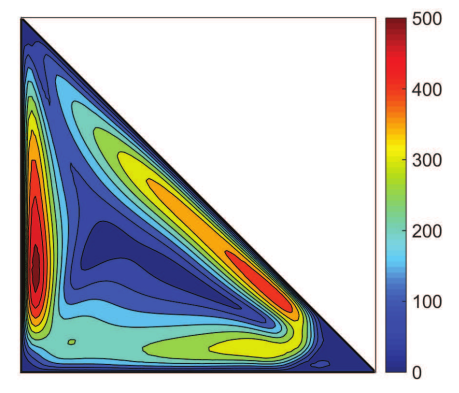
\includegraphics[width=4.5cm]{python_codes/fieldstone_51/images/jolm17_vel}
b)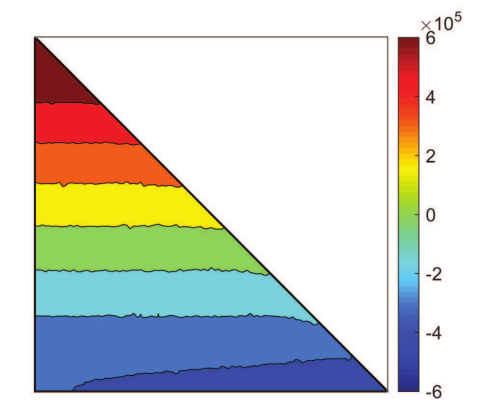
\includegraphics[width=4.5cm]{python_codes/fieldstone_51/images/jolm17_p}
c)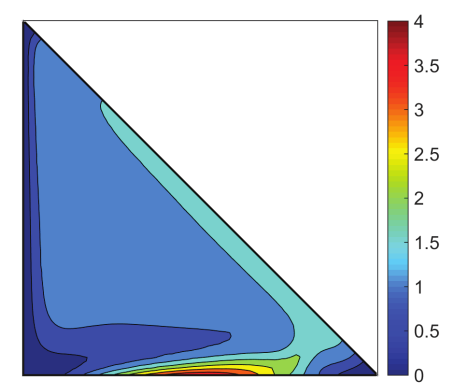
\includegraphics[width=4.5cm]{python_codes/fieldstone_51/images/jolm17_T}\\
{\small Steady state fields: a) velocity, b) pressure, c) temperature.}
\end{center}

Although it is not mentioned in the original article it appears that the 
pressure field has been normalised so that $\langle p \rangle = \int_\Omega p dV=0$.

As opposed to the mesh presented in \cite{jolm17} I build a regular mesh.
An example of such a mesh is shown hereunder (a) for $n=5$ (the number of nodes
per side of the triangular domain). 
In order to generate a mesh which is more isotropic some edges between 
triangles can be flipped (b). 
Note that this mesh can also be modified in such a way that the position of 
nodes inside the domain is perturbed by a small random value (c).
In what follows I denote by $h$ the distance between nodes
on the horizontal (or vertical) boundaries, i.e. $h=L_x/(n-1)=L_y/(n-1)$.
\begin{center}
a)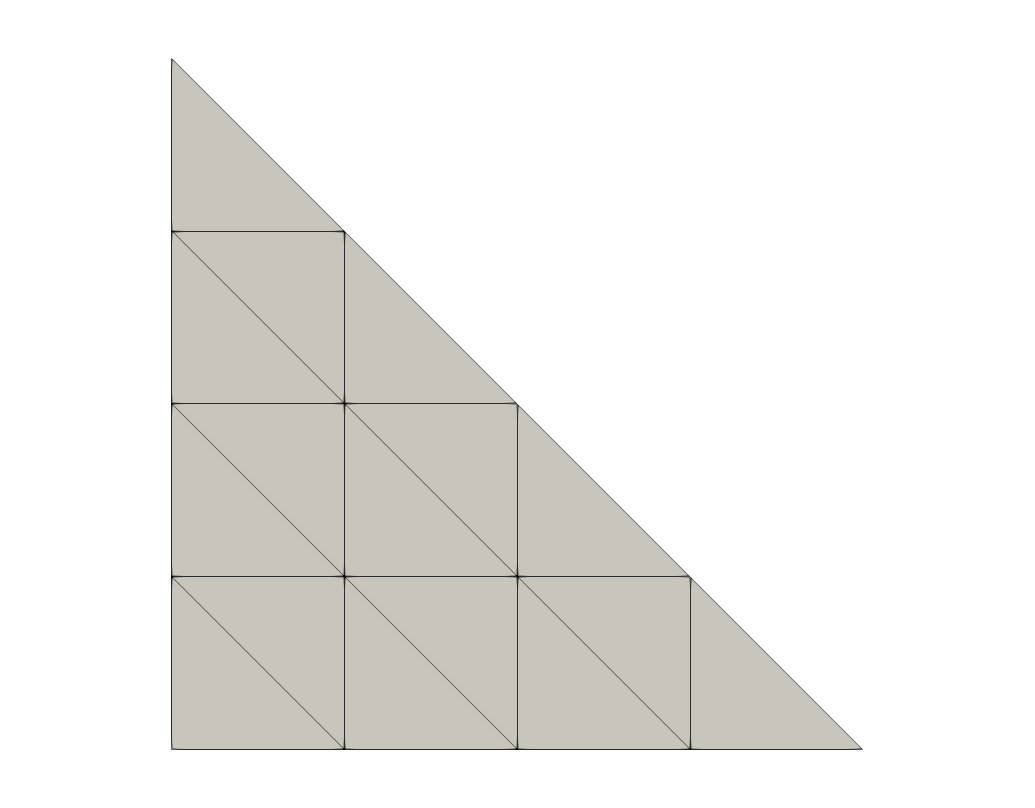
\includegraphics[width=4.5cm]{python_codes/fieldstone_51/images/minigrid5a}
b)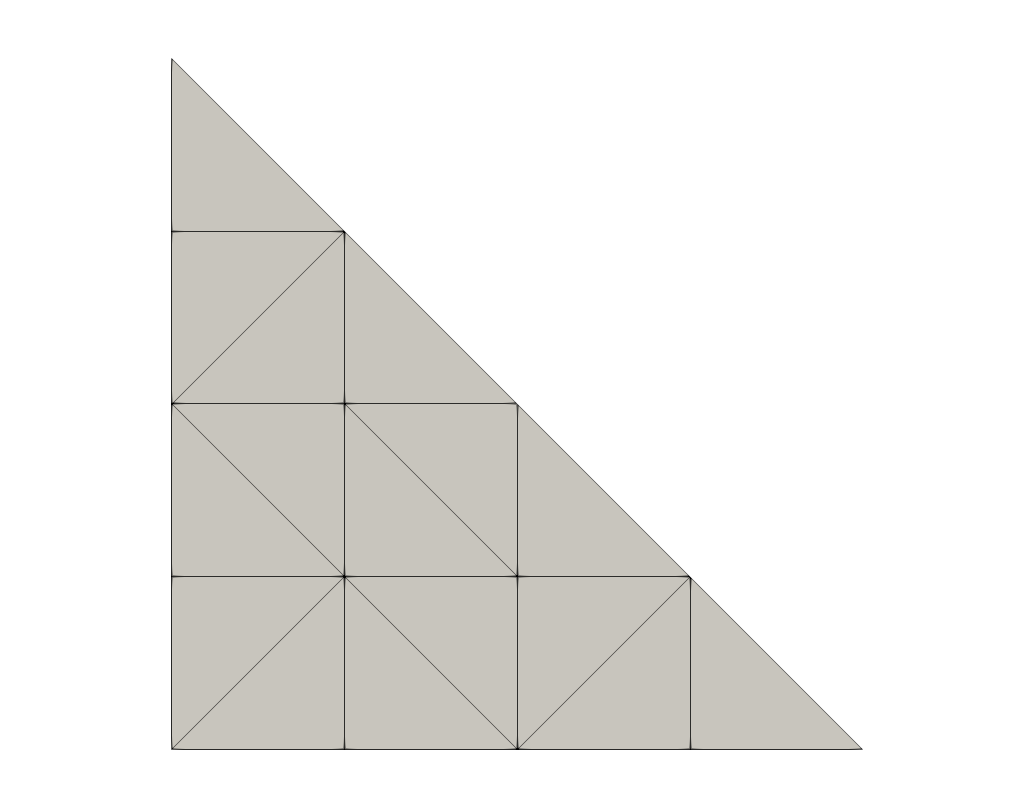
\includegraphics[width=4.5cm]{python_codes/fieldstone_51/images/minigrid5b}
c)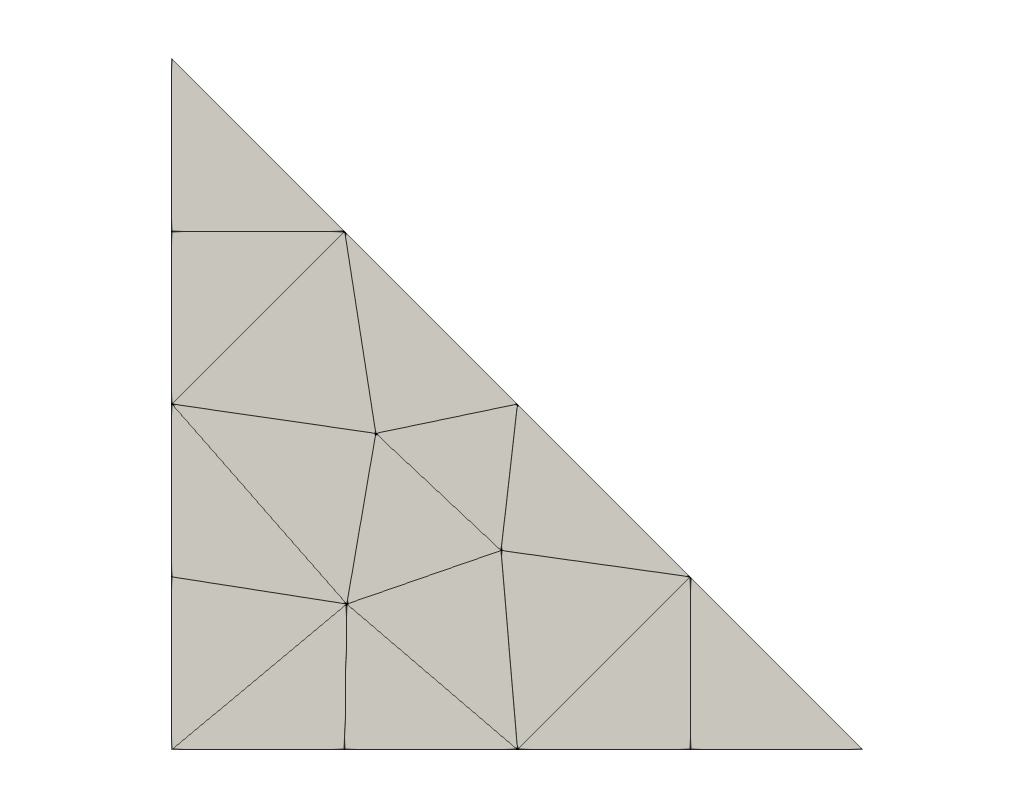
\includegraphics[width=4.5cm]{python_codes/fieldstone_51/images/minigrid5c}\\
{\small a) regular mesh for n=5. b) flipped edges mesh. c) randomized+flipped edges mesh.}
\end{center}

Since I am solving for the steady-state solution I set the mass matrix in the 
heat transport part of the code to zero. However, since I am solving the stokes equations
and the heat transport equation alternatively until convergence is reached, it is well 
known that this approach does not converge fast (if at all). 
I then implement a simple relaxation scheme \cite{vyrc13}. After I have solved for velocity (using the 
most recent temperature field in the rhs), I do:
\[
\vec{v}^k = \gamma \vec{v}^k + (1-\gamma) \vec{v}^{k-1}
\]
and after having solved for temperature having used the most recent velocity field, 
I do the same for temperature:
\[
{T}^k = \gamma {T}^k + (1-\gamma) {T}^{k-1}
\]
where the relaxation parameter $\gamma$ is between 0 and 1.




Additionally I measure:
\begin{itemize}
\item the Nusselt number defined by 
\[
Nu
=\int_{y=0} \vec{\nabla}T \cdot \vec{n} dS  
=-\int_{x=0}^{x=1} \frac{\partial T}{\partial y} dx 
\]
It is reported to be 24.535 in \cite{jolm17}.
\item the temperature on the hypotenuse.
\item the root mean square velocity
\item the mean temperature $\langle T \rangle = |\Omega|^{-1} \int_\Omega T \; dV$
\end{itemize}

%----------------------------------------------------------------------
\subsubsection*{On the importance of the relaxation parameter $\gamma$}

In what follows the internal node coordinate randomness is switched off.
I have run the model for various values of $\gamma$ for $n=25$, and results are shown on the 
following figures. We see that all simulations seem to converge to the same 
steady state, which is very reassuring. However, it looks like too small a value of $\gamma$
delays greatly the convergence and too large a value also seems detrimental. 
In light of this, I have chosen $\gamma=0.2$ for all what follows.

\begin{center}
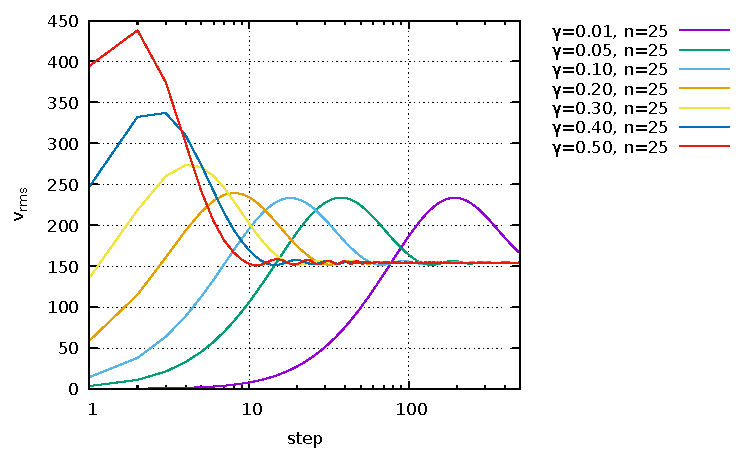
\includegraphics[width=5cm]{python_codes/fieldstone_51/images/vrms_gammas.pdf}
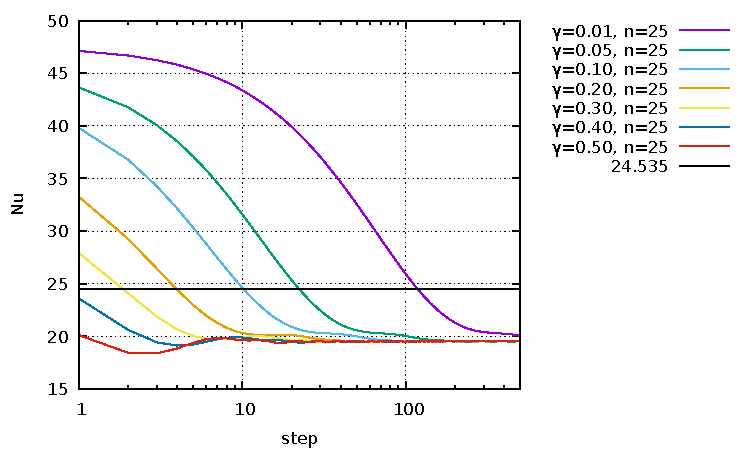
\includegraphics[width=5cm]{python_codes/fieldstone_51/images/Nu_gammas.pdf}
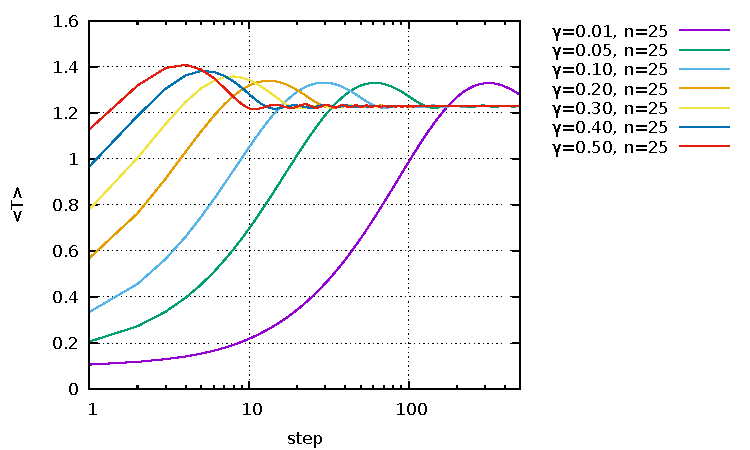
\includegraphics[width=5cm]{python_codes/fieldstone_51/images/avrgT_gammas.pdf}\\
{\small Left to right: Root mean square velocity, Nusselt number and average temperature as a function 
of the iteration counter.}
\end{center}

%----------------------------------------------------------------------
\subsubsection*{On the influence of mesh resolution} 

I now explore the influence of the mesh resolution on the results and run steady state 
calculations for $n=25,50,75,100$.

\begin{center}
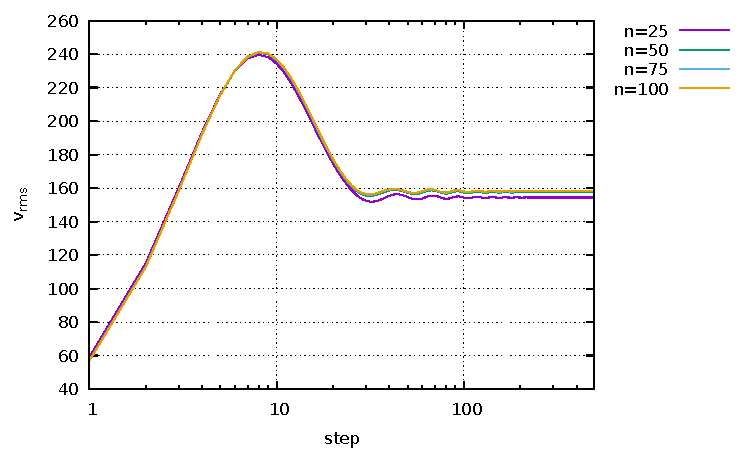
\includegraphics[width=7cm]{python_codes/fieldstone_51/images/vrms_res.pdf}
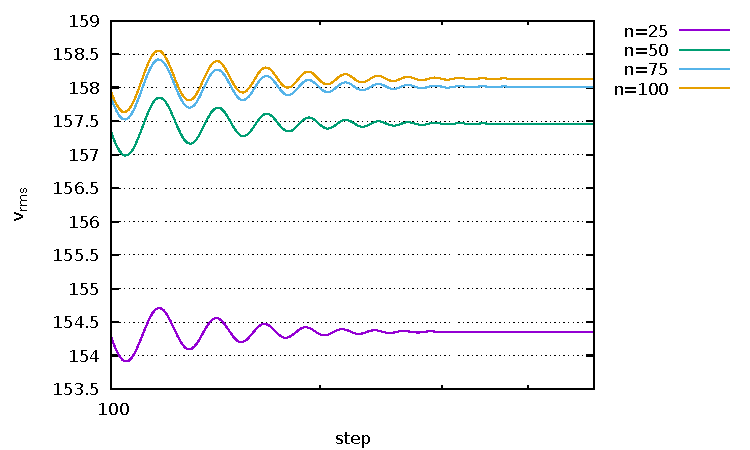
\includegraphics[width=7cm]{python_codes/fieldstone_51/images/vrms_res_zoom.pdf}\\
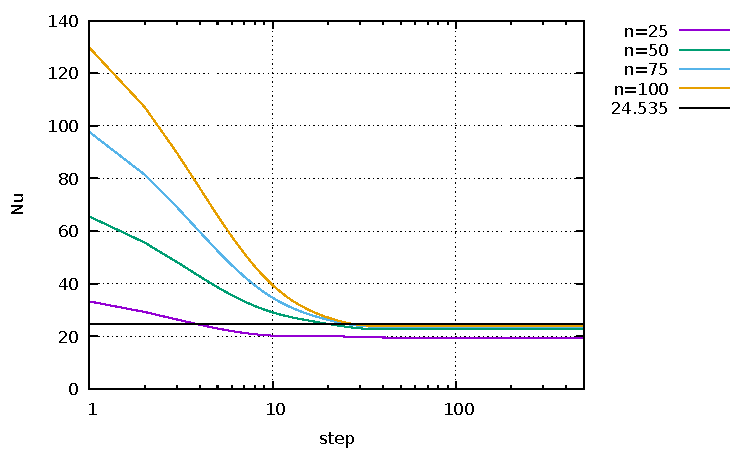
\includegraphics[width=7cm]{python_codes/fieldstone_51/images/Nu_res.pdf}
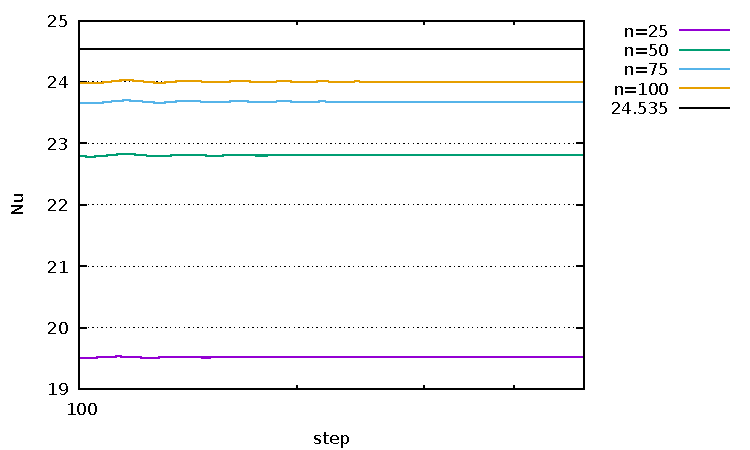
\includegraphics[width=7cm]{python_codes/fieldstone_51/images/Nu_res_zoom.pdf}\\
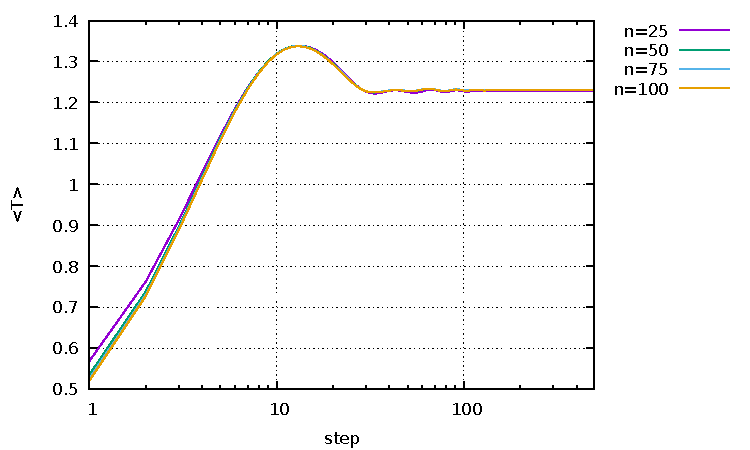
\includegraphics[width=7cm]{python_codes/fieldstone_51/images/avrgT_res.pdf}
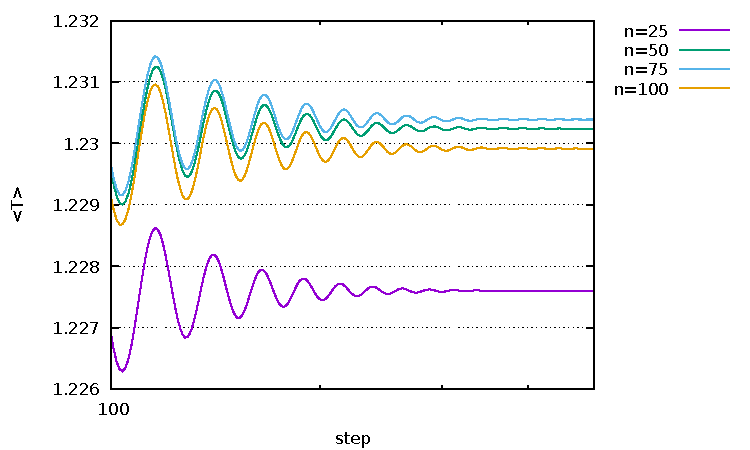
\includegraphics[width=7cm]{python_codes/fieldstone_51/images/avrgT_res_zoom.pdf}\\
\end{center}

\begin{center}
\begin{tabular}{llll}
\hline
resolution $(n)$ & $v_{rms}$ & Nu & $\langle T \rangle$ \\
\hline
\hline
25  & 154.35406 & 19.51906 &  1.22759\\
50  & 157.46000 & 22.80683 &  1.23024\\
75  & 158.01207 & 23.67889 &  1.23038\\
100 & 158.13157 & 24.00510 &  1.22991\\
\hline
\end{tabular}
\end{center}

The following two plots show the temperature along the hypotenuse (as a function of $x$
for simplicity) at steady-state and the heat flux measured at the bottom. 
\begin{center}
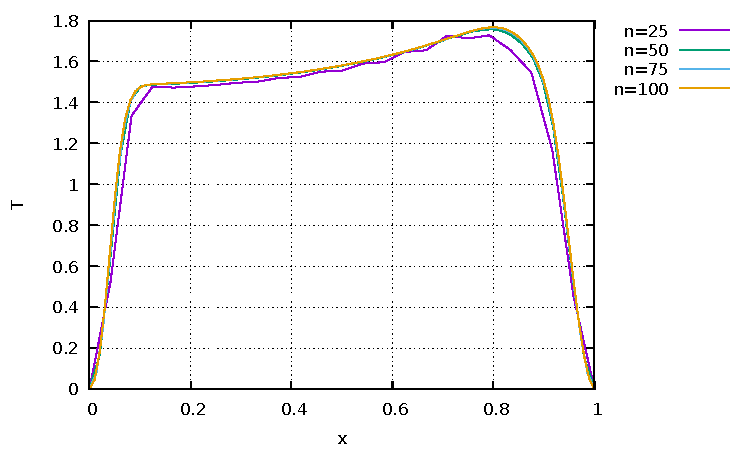
\includegraphics[width=7cm]{python_codes/fieldstone_51/images/temp_hyp_res.pdf}
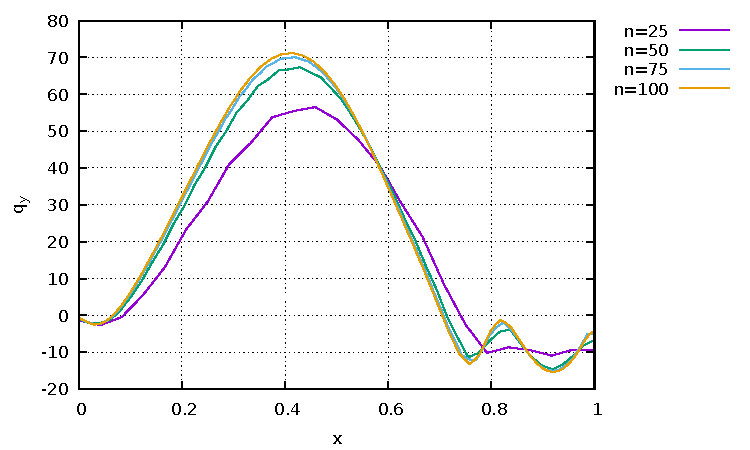
\includegraphics[width=7cm]{python_codes/fieldstone_51/images/qy_bot_res.pdf}
\end{center}

Finally, here are the fields for $n=100$ at steady state:

\begin{center}
a)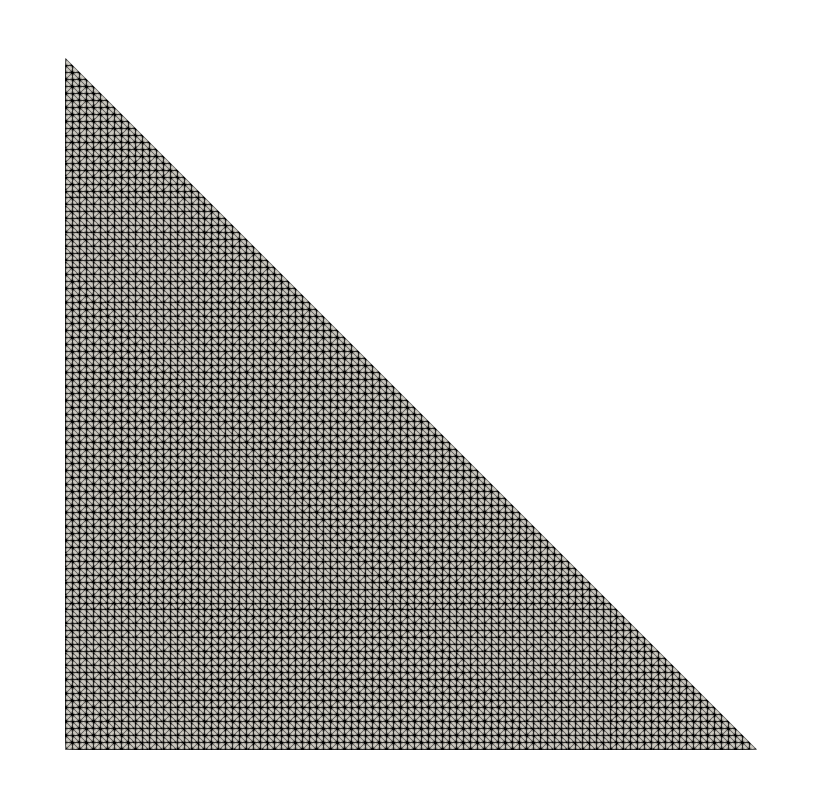
\includegraphics[width=4.5cm]{python_codes/fieldstone_51/images/relax0p20_100/grid}
b)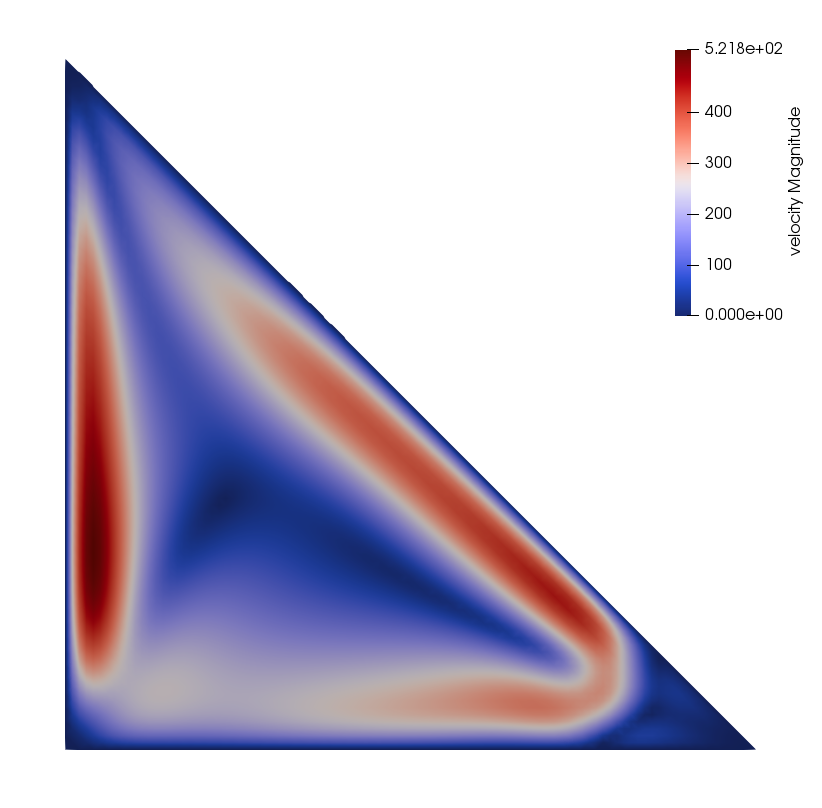
\includegraphics[width=4.5cm]{python_codes/fieldstone_51/images/relax0p20_100/vel}
c)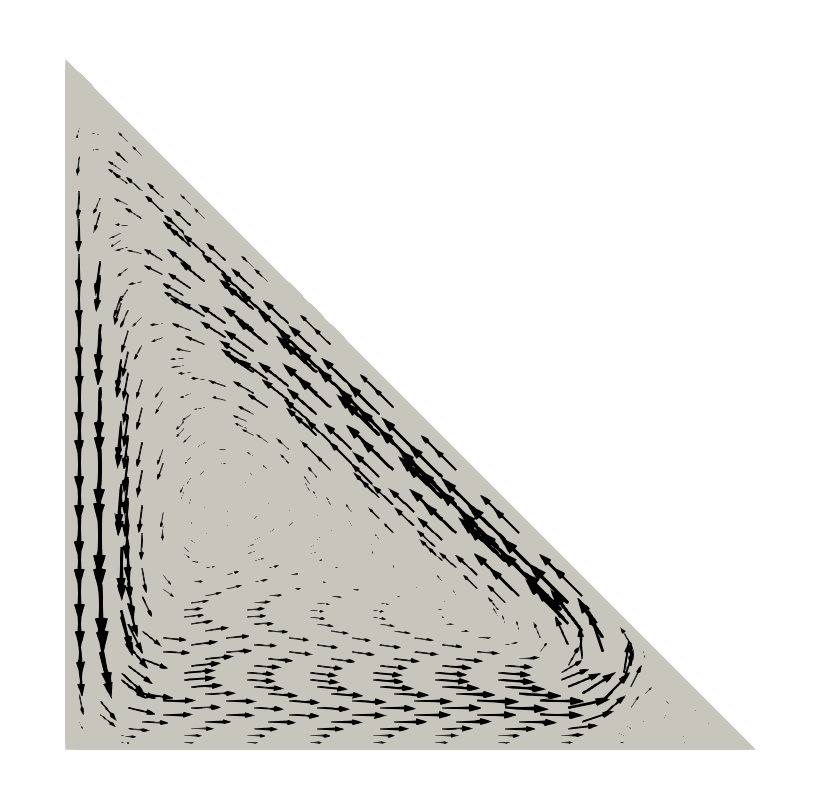
\includegraphics[width=4.5cm]{python_codes/fieldstone_51/images/relax0p20_100/vel2}\\
d)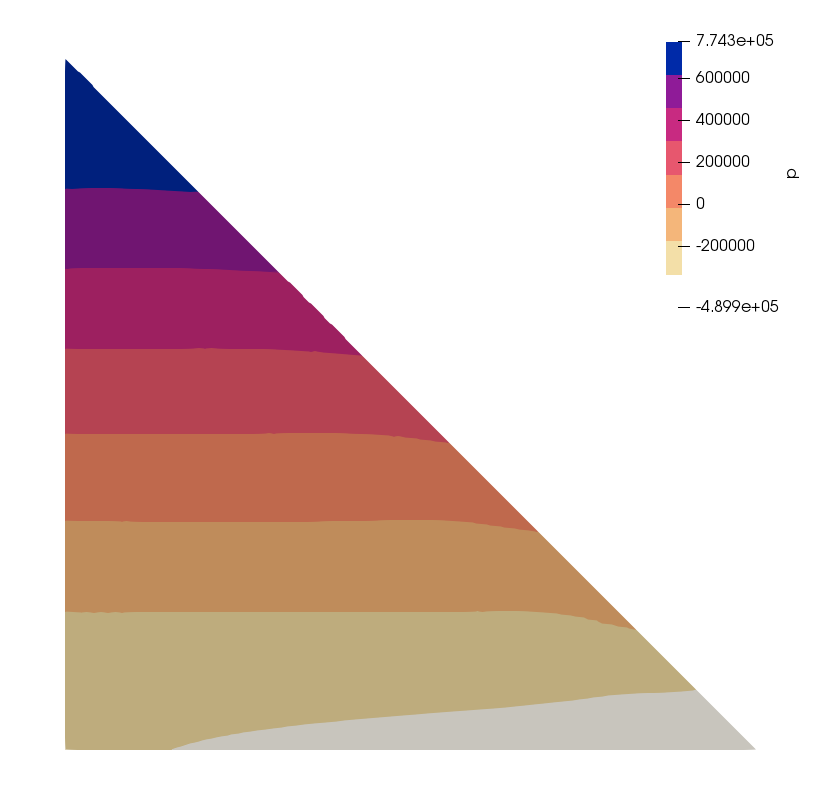
\includegraphics[width=4.5cm]{python_codes/fieldstone_51/images/relax0p20_100/p}
e)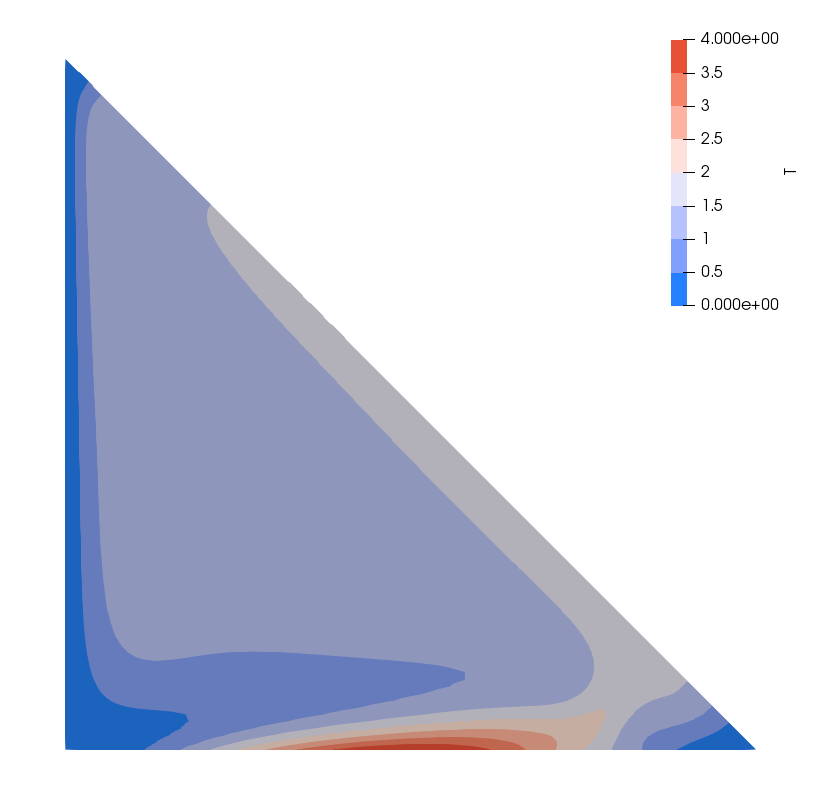
\includegraphics[width=4.5cm]{python_codes/fieldstone_51/images/relax0p20_100/T}
f)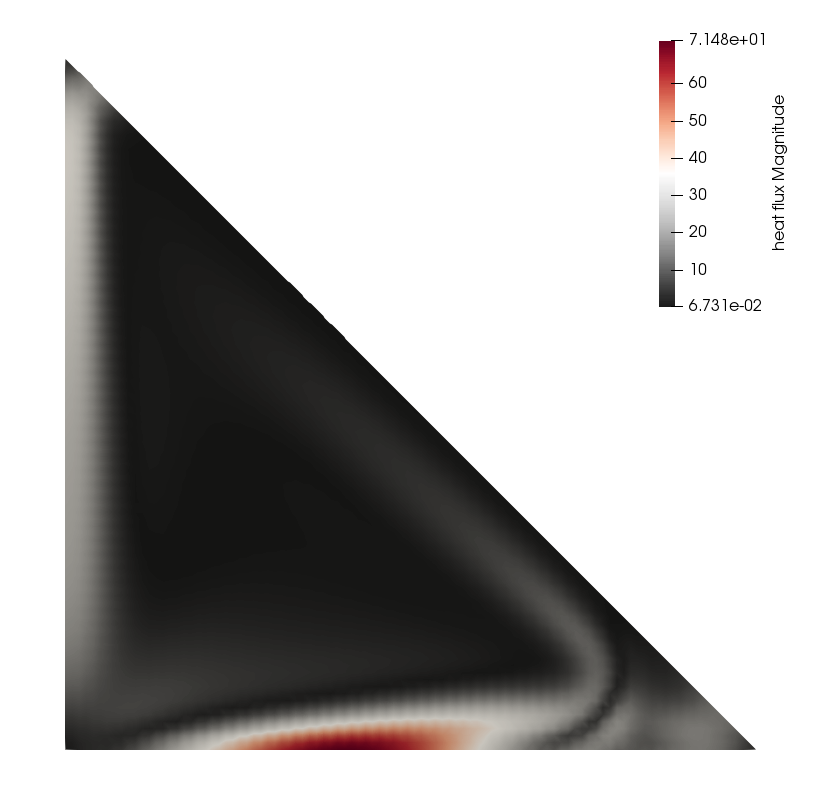
\includegraphics[width=4.5cm]{python_codes/fieldstone_51/images/relax0p20_100/heatflux}\\
g)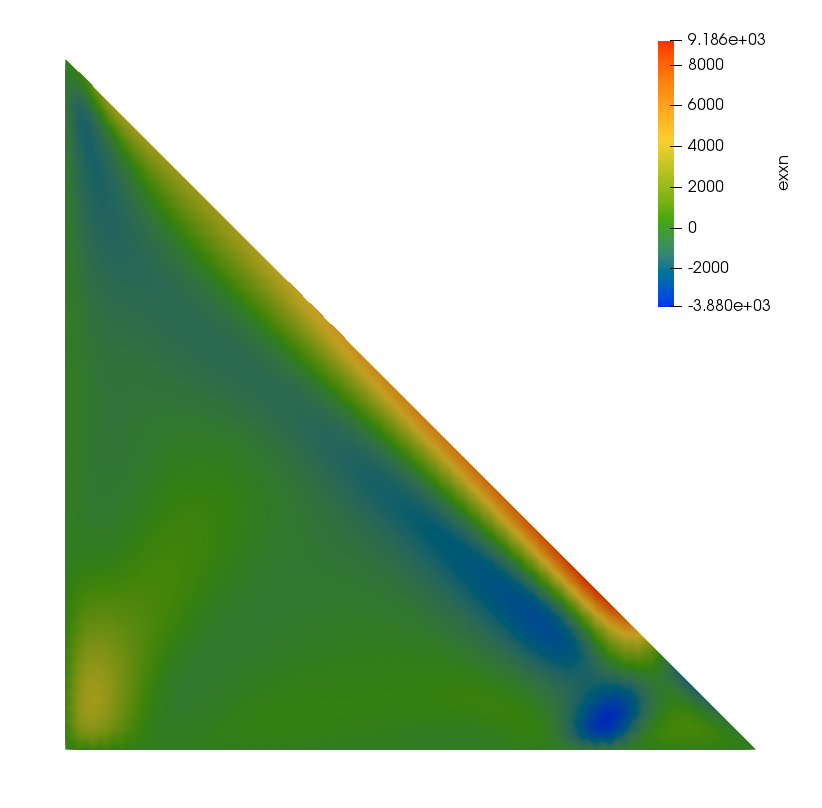
\includegraphics[width=4.5cm]{python_codes/fieldstone_51/images/relax0p20_100/exx}
h)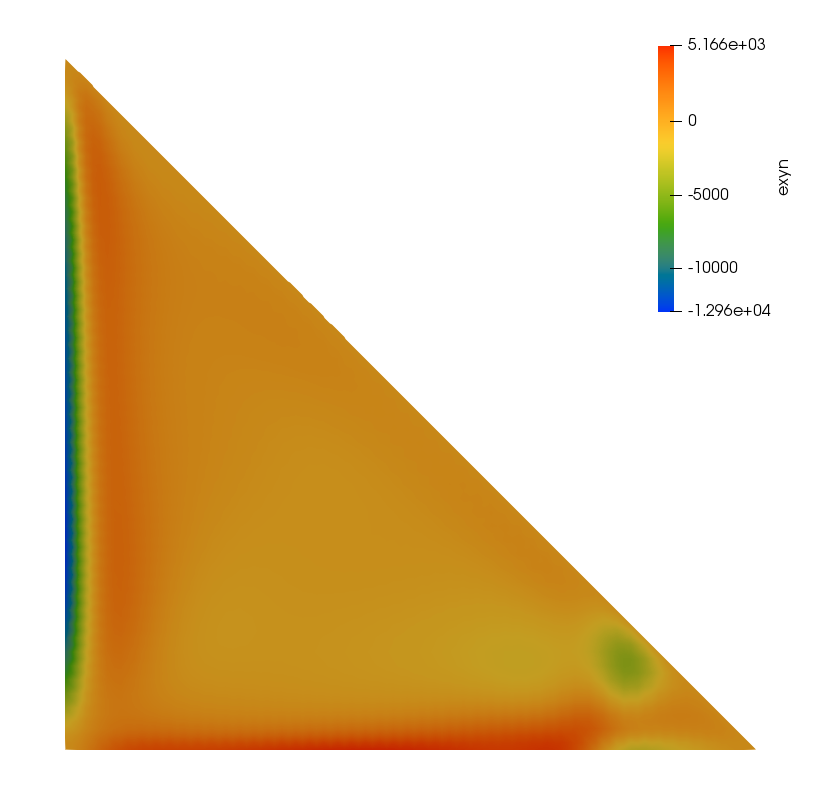
\includegraphics[width=4.5cm]{python_codes/fieldstone_51/images/relax0p20_100/exy}
i)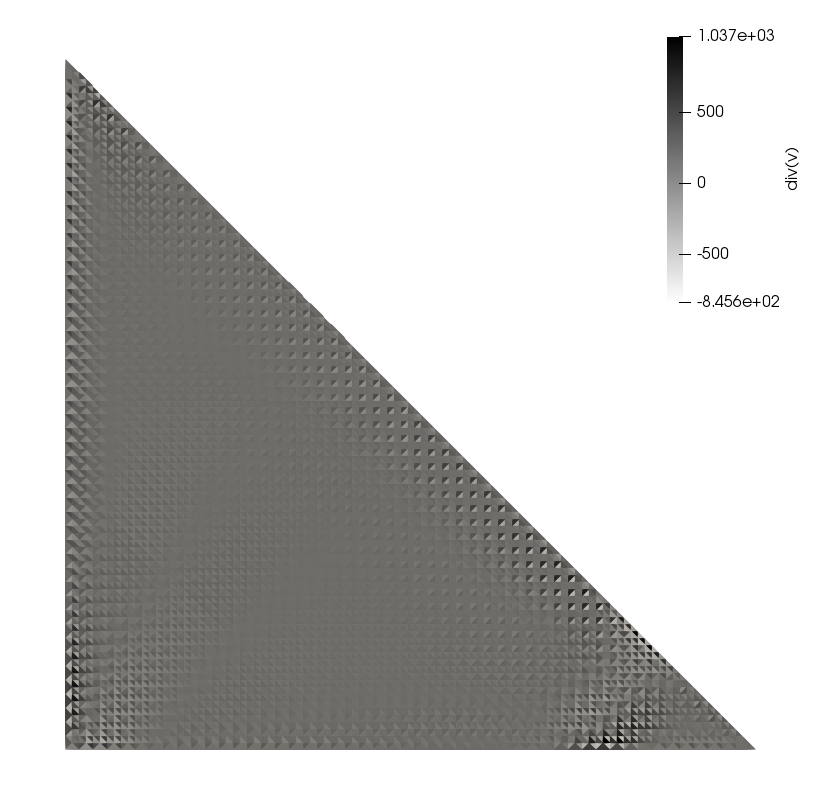
\includegraphics[width=4.5cm]{python_codes/fieldstone_51/images/relax0p20_100/divv}\\
{\small Steady state fields: a) grid (n=100), b,c) velocity, d) pressure, e) temperature,
f) heat flux, g) $\dot{\varepsilon}_{xx}$, h) $\dot{\varepsilon}_{xy}$, i) velocity 
divergence measured in the middle of the element.}
\end{center}




